\documentclass[conference]{IEEEtran}
\usepackage[pdftex]{graphicx}
\graphicspath{{images/}}
\DeclareGraphicsExtensions{.pdf,.jpeg,.png}

\hyphenation{op-tical net-works semi-conduc-tor}

\begin{document}

\title{CarSensor: Smart Street-side Parking with the Internet of Things}


% author names and affiliations
% use a multiple column layout for up to three different
% affiliations
\author{\IEEEauthorblockN{Daniel Lynch}
	\IEEEauthorblockA{Deparment of Mechanical Engineering\\
		Northwestern University\\
		2145 Sheridan Road\\
		Evanston, IL 60208, USA\\
		\texttt{daniellynch2021@u.northwestern.edu}}
	\and
	\IEEEauthorblockN{Yong Zhao}
	\IEEEauthorblockA{MPM Program\\
		Northwestern University\\
		2145 Sheridan Road\\
		Evanston, IL 60208, USA\\
		\texttt{yongzhao2019@u.northwestern.edu}}
	}
	
\maketitle

\begin{abstract}
	The abstract goes here.
	No, it goes here.
\end{abstract}

\section{Introduction}
The recent surge in popularity of the Internet of Things (IoT) highlights some fundamental aspects of the design and analysis of cyberphysical systems, such as deterministic behavior, robustness, and extensibility. For the final project of EECS 395/495 Cyberphysical Systems (Winter 2018), we created \texttt{CarSensor}, a prototype of an IoT-inspired system for smarter street-side parking, which addressed these aforementioned aspects of cyberphysical systems.

\subsection{Use Case}
Parking on the street can be a hassle, especially in urban areas. Knowing which parking spaces are full or empty can save a lot of time and aggravation. One way to realize this is by outfitting a street with an IoT system consisting of networked sensors and a client application all communicating with a central hub.

\subsection{Physical Layout}
\begin{figure}[h]
\centering
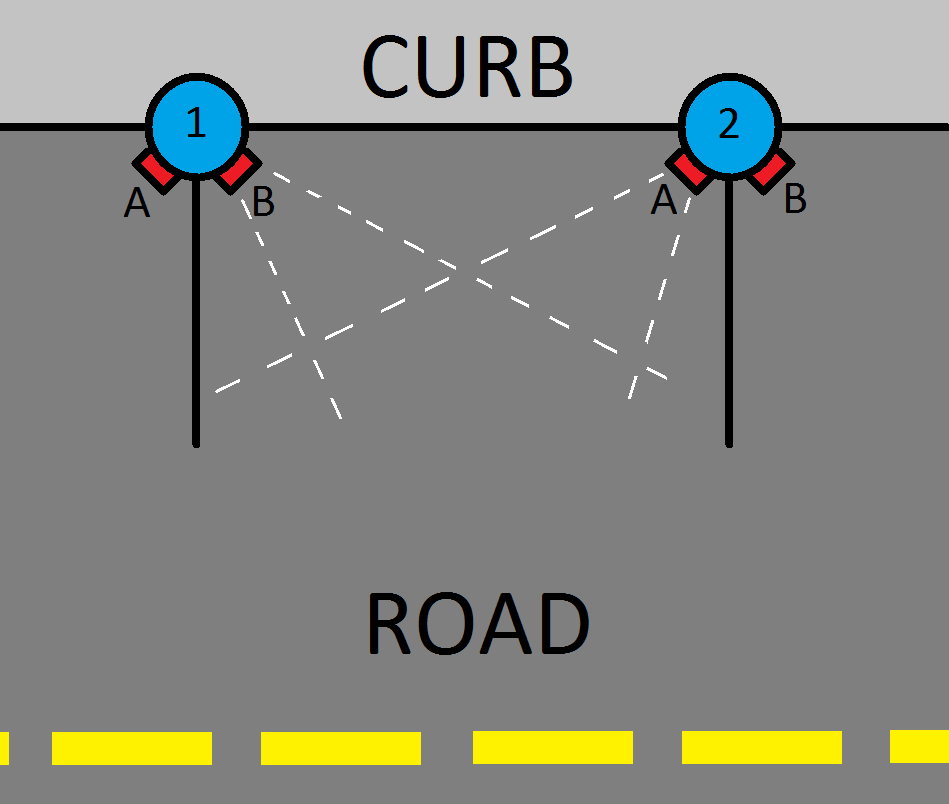
\includegraphics[width=2.0in]{parkingspace.png}
\caption{Simulation results for the network.}
\label{fig_curb}
\end{figure}

\section{Physical Layer}

\section{Network Layer}
\subsection{Sensor Clients}
\subsection{Server}
\subsubsection{State Machine}
\begin{figure}[h]
	\centering
	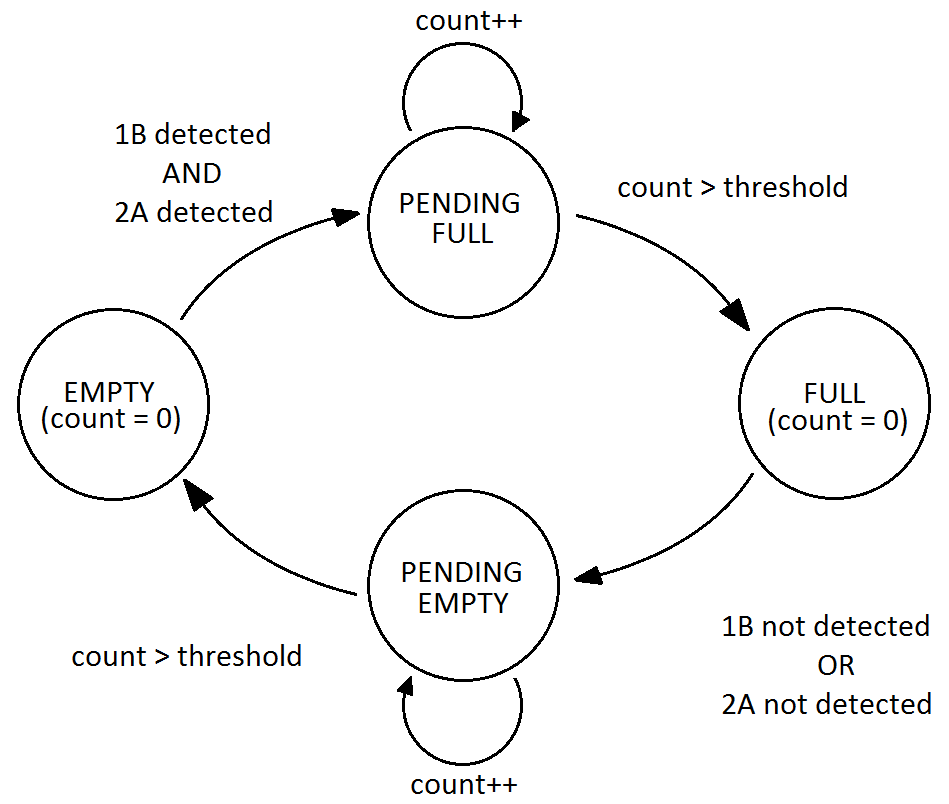
\includegraphics[width=2.0in]{FSM.png}
	\caption{Simulation results for the network.}
	\label{fig_fsm}
\end{figure}
\subsection{App Client}

\end{document}